\section{Experimental Constraints}
Unfortunately it is extremely difficult to obtain a real space image of the spin configurations of these 3-D magnetic pyrochlore oxide structures without altering the state the system is in. However there have been numerous experiments recently concentrating on `artificial' 2-D spin ice and also simulations. These materials are artificially produced and lithographically fabricated isolated single-domain nano-magnets arranged in regular lattice such as the square lattice and the kagome lattice which I will be concentrating on in this report.{\cite{b13}}
\par
\subsection{Square Lattice}
In the case of the square lattice, the islands have intrinsic magnetic moments and the shape anisotropy of the islands effectively force these moments to point along the long axis of the islands as opposed to 3-D spin ice where it is the magneto crystalline anisotropy which determines the direction of the moments.
\par
We can now consider the moments to be Ising like as they only have two states available to them, parallel or anti-parallel to their long axis. This lattice construction enables the study of dipole interactions between islands creating a simpler 2-D analogue to the more complicated and difficult to study 3-D pyrochlore oxides.
\par
Important notes to make here are that the islands are isolated in that they are not physically connected to one another and considering a single vertex of the lattice it obeys the ice rules of 2 in 2 out.  The advantage of working with artificial spin ice is that it's possible to experimentally image the lattices using imaging techniques such as Atomic force microscopy, Magnetic Force Microscopy or X-ray Magnetic Circular Dichroism and that in the majority of cases these imaging processes can be performed at room temperature.
\par
\begin{figure}[ht!]
    \begin{center}
        \subfloat[Atomic force microscopy][Atomic force microscopy]{
        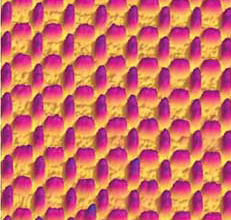
\includegraphics[width=0.35\textwidth]{afm.png}
        \label{fig:sf5.1}}
\qquad
        \subfloat[Magnetic force microscopy][Magnetic force microscopy]{
        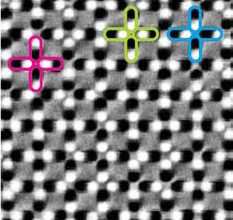
\includegraphics[width=0.35\textwidth]{mfm.png}
        \label{fig:sf5.2}}
        \caption[Imaging techniques used by R.F. Wang et al.]{Square spin ice lattice images}
        \label{fig:gf5}
    \end{center}
\end{figure}
Some such images from the experiments carried out by R.F. Wang et al. on a square lattice are shown in Figure 6.  The lattice spacing in both images is 400nm and the islands are 220nm $\times$ 80nm in size.{\cite{b13}
\clearpage
\subsection{Frustration on the Kagome Lattice}
Unfortunately the origin of frustration in the square lattice is not geometric like it is in the 3-D pyrochlore lattice.  There is, however, a structure in which the frustration is an inherent property due to the geometry and therefore creates a more accurate 2-D analogue to the 3-D pyrochlore lattice and this structure is the 2-D kagome lattice.
\par
\begin{figure}[ht!]
    \begin{center}
        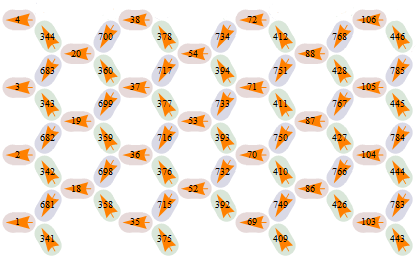
\includegraphics[scale=1.00]{kaglatsam.png}
        \caption[Kagome lattice sample]{Kagome lattice sample}
        \label{fig:gf6}
    \end{center}
\end{figure}
The Monte Carlo simulations in this experiment were performed on a 2-D Kagome lattice such as that shown in Figure 6 above. It is important to note that, similar to the experiments on the square lattice, the islands share no connections with neighbouring islands or in other words are `isolated' and the dipoles are limited to point in two directions parallel or anti-parallel to their long axis.
\par
\begin{figure}[ht!]
    \begin{center}
        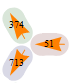
\includegraphics[scale=1.4]{kagbasunit.png}
        \caption[Basic kagome lattice unit]{Basic kagome lattice unit}
        \label{fig:gf7}
    \end{center}
\end{figure}
If we examine for a moment the basic unit of the kagome lattice,  it is composed of 3 dipoles converging at a vertex as shown in Figure 8 above.  Consider that each dipole's magnetic moment to be stretched into a charged dumbbell with the charges $\pm$q residing at the opposite ends.  This is known as the charge model.  Then at the vertex in this basic unit the ground state can be one of two values : $\pm$q.
\par
These vertex have an inherently frustrated or degenerate ground state that can take one of two forms : 2 in 1 out, giving +q or 1 in 2 out, giving -q. In the case of the above figure 8 the `charge' at the vertex would be $-$q.
\clearpage
